\documentclass[12pt]{article}

\usepackage{xcolor}
\usepackage{listings}
\usepackage{hyperref}
\usepackage{pdfpages}

\hypersetup{
    colorlinks=true,
    linkcolor=blue,
    filecolor=magenta,      
    urlcolor=cyan,
    pdftitle={HW07},
    pdfpagemode=FullScreen,
    }
\lstset{basicstyle=\ttfamily,
showstringspaces=false,
commentstyle=\color{red},
keywordstyle=\color{blue}
}

\renewcommand{\thesubsection}{\thesection.\alph{subsection}}

\title{Programming Assignment 7 \\ \small{ECE 759, Prof. TW Huang}}
\author{Sai Tadinada}
\date{}

\begin{document}
\maketitle

GitHub link to programming tasks: \\ \url{https://github.com/phantom3012/repo759/tree/main/HW07}

\section{Question 1}

\subsection{}
\texttt{task1.cu} can be found at \url{https://github.com/phantom3012/repo759/blob/main/HW07/task1.cu}

\subsection{}
Scaling analysis plot for task1 is shown as in Figure \ref{fig:task1}:
\begin{figure}[ht]
    \centering
    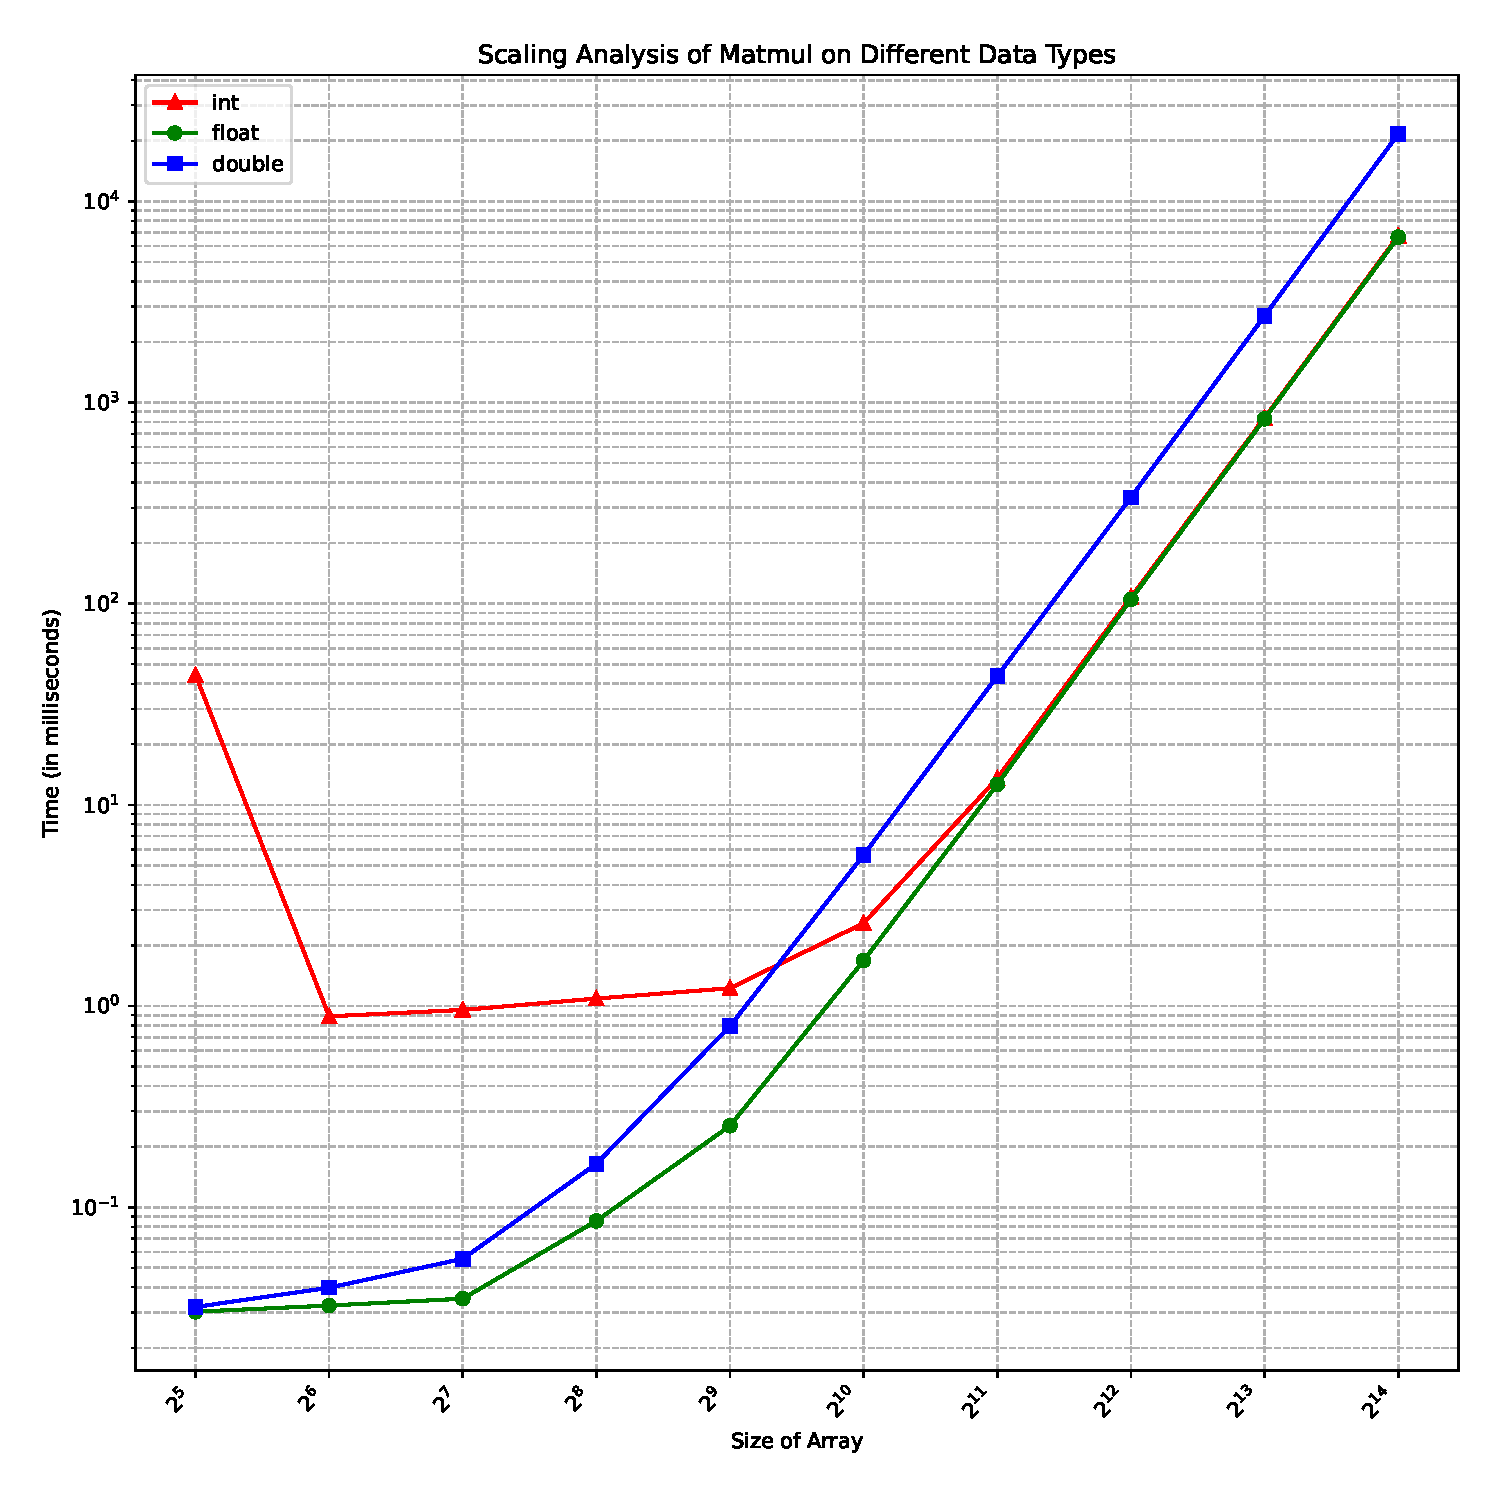
\includegraphics[width=0.8\textwidth]{task1.pdf}
    \caption{Scaling Analysis for task1 (matrix multiplication)}
    \label{fig:task1}
\end{figure}

\subsection{} % best possible value of block_dim for n = 2^14
The best possible value of \texttt{block\_dim} for $n = 2^{14}$ is 32.
\subsection{} % performance change betweeen types of data
The performance of the code is better when using \texttt{float} data type compared to \texttt{double} data type. This is because \texttt{float} data type requires less memory and hence, the number of operations required to perform the matrix multiplication is less compared to \texttt{double} data type.
\subsection{} % runtime diff in HW07 vs HW06
In the naive implementation, the runtime for the matmul function is 52469.1ms as compared to the tiled implementation which results in a time of 21599.4 ms. The tiled implementation is faster by a factor of 2.43 simply due to the fact that the memory access pattern is more efficient in the tiled implementation.
\subsection{} % CPU vs GPU of matmul on n = 2^14
The CPU implementation times out after 10 minutes whereas the GPU implementation takes 21599.4 ms. The GPU implementation is faster and more efficient because of the exploitation of parallelism in the GPU.


\clearpage
\section{Question 2}

\subsection{}
\texttt{task2.cu} can be found at \url{https://github.com/phantom3012/repo759/blob/main/HW07/task2.cu}

\subsection{}
Scaling analysis plot for task2 is shown below:
\begin{figure}[ht]
    \centering
    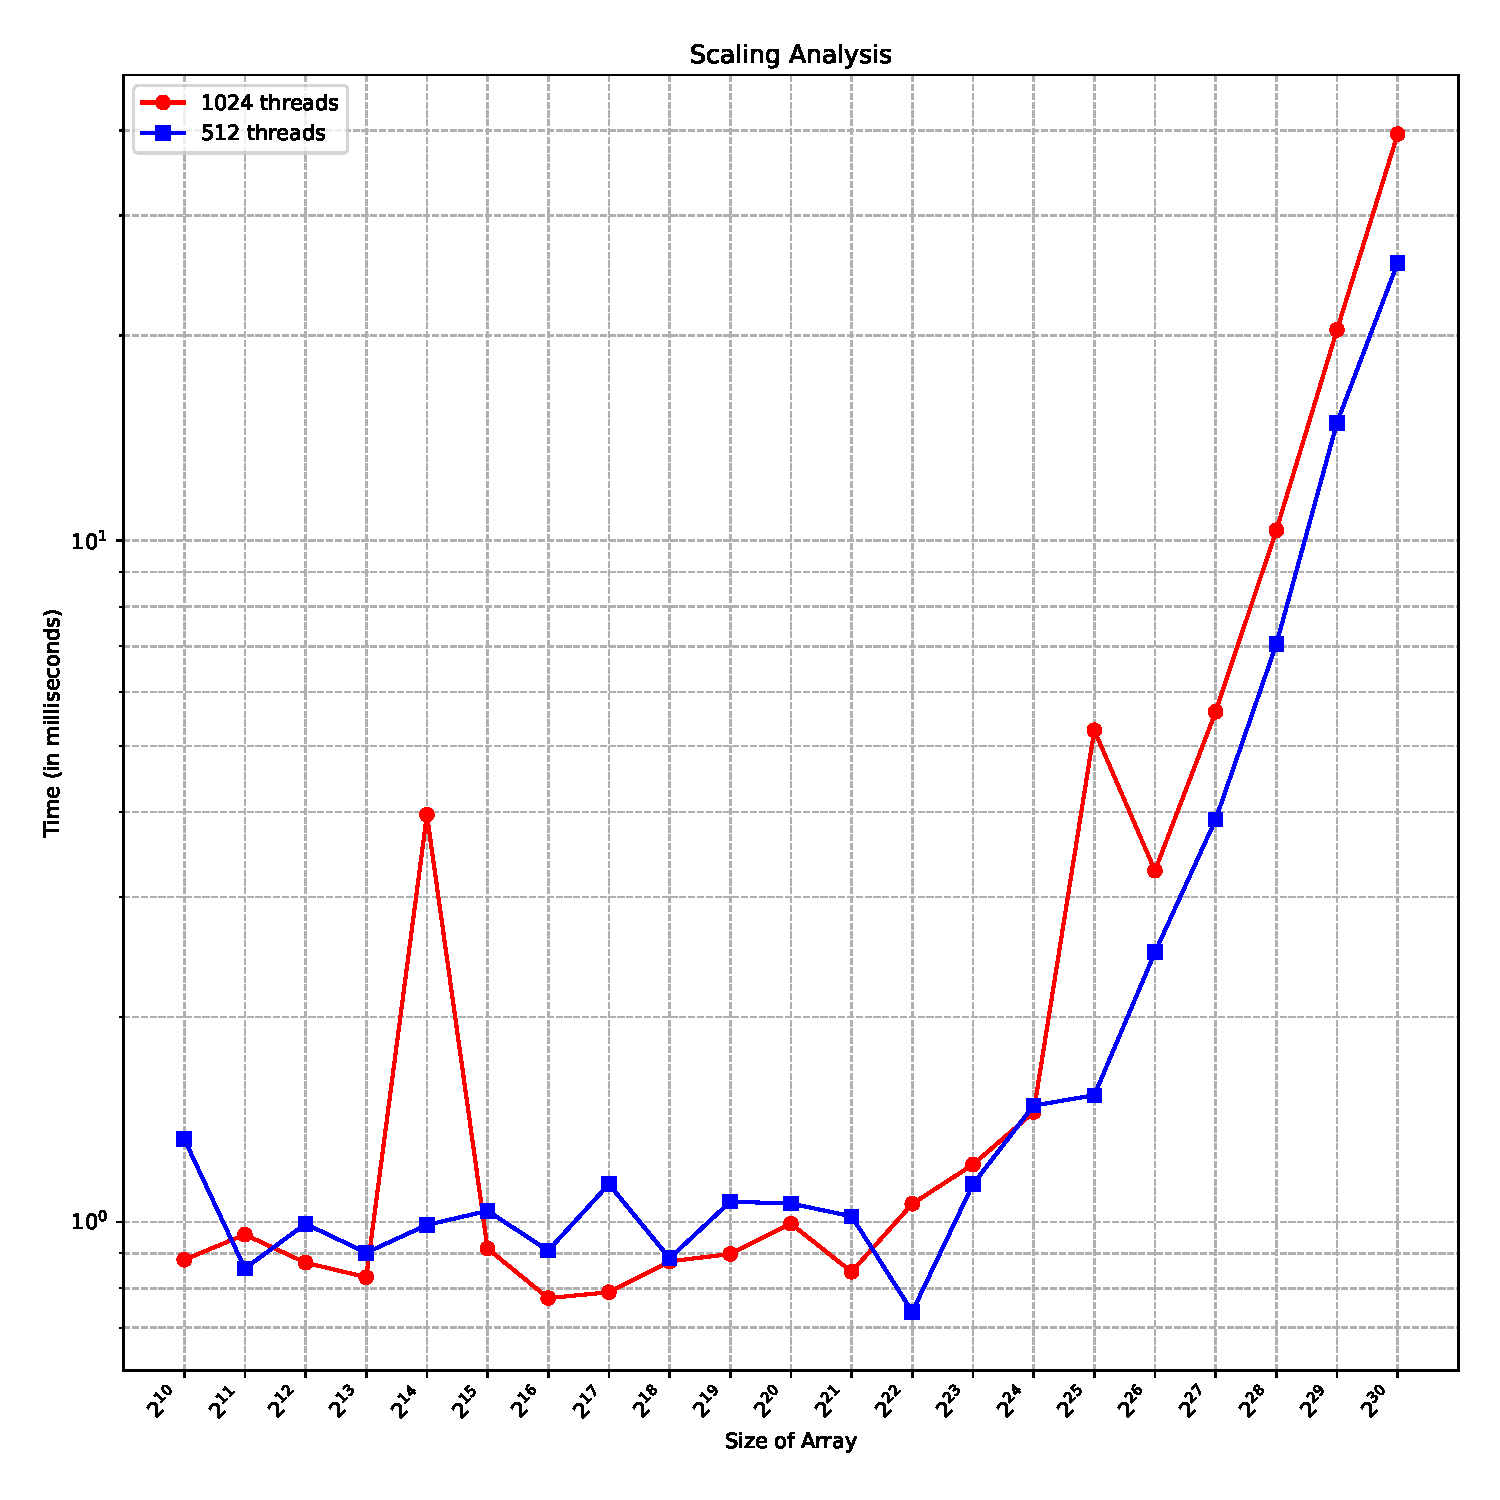
\includegraphics[width=0.7\textwidth]{task2.pdf}
    \caption{Scaling Analysis for task2 (reduction)}
\end{figure}


\end{document}